\chapter{Численный метод}\label{ch:numeric}
В ходе исследования были произведены вычисления в двух моделях: сплошной среды и системы тонких нитей.

\section{Модель сплошной среды}\label{sec:model-simple}
Для расчётов в модели сплошной среды для описания состояния используются следующие переменные:

\begin{gather*}
    u_{\alpha} - компоненты~вектора~скорости \\
    \sigma_{\alpha\beta} - компоненты~тензора~напряжений \\
    \rho - плотность~материала \\
    \varepsilon - внутренняя~энергия
\end{gather*}

Материал принимается упруго-пластическим.
Основная система уравнений имеет вид:

\begin{equation}
    \frac{d\rho}{dt} + \rho \frac{\partial u_{\alpha}}{\partial x_{\alpha}} = 0
\end{equation}
\begin{equation}
    \frac{d u_{\alpha}}{dt} - \frac{1}{\rho} \frac{\partial \sigma_{\alpha \beta}}{\partial x_{\beta}} = 0
\end{equation}
\begin{equation}
    \frac{de}{dt} = \frac{1}{\rho} \sigma_{\alpha \beta} \varepsilon_{\alpha \beta}
\end{equation}

В данной записи $\varepsilon_{\alpha \beta}$ -- компоненты тензора скоростей деформации.
Производная по времени берётся в движущейся СК (производная Лагранжа), так как это упростит формулировку численного метода.

Для описания поведения материала используется гиперупругое соотношение:
\begin{equation}
    \frac{d S_{\alpha \beta}}{d t} = 2 \mu \left( \varepsilon_{\alpha \beta} - \\
    \frac{1}{3} \delta_{\alpha \beta} \varepsilon_{\alpha \beta} \right) + S_{\alpha \gamma} R_{\beta \gamma} + \\
    S_{\gamma \beta} R_{\alpha \gamma}
\end{equation}
С формулировкой через девиатор напряжения $S_{\alpha\beta}$:
\begin{equation}
    R_{\alpha \beta} = \frac{1}{2} \left( \frac{\partial u_{\alpha}}{\partial x_{\beta}} + \frac{\partial u_{\beta}}{\partial x_{\alpha}} \right)
\end{equation}

Режим пластического деформирования материала в данной работе описывается на основании теории Прандтля-Рейсса.
В качестве критерия перехода из упругого состояния в пластическое течение выбирается критерий Мизеса, основанный
на энергии изменения формы (сдвиговых деформациях).
Математическая формулировка критерия фиксирует переход к пластическому деформированию при выполнении условия
$s = S_{\alpha \beta} S_{\alpha \beta} = 2 K^2$.
Внутри поверхности $s < 2 K^2$ поведение материала при нагружении считается линейно-упругим.
Вне указанной поверхности для учёта необратимых деформаций и течения материала в уравнение вводится член:
$-\theta(s)(S_{\alpha \beta}\varepsilon_{\alpha \beta})S_{\alpha \beta}$, где
\begin{equation}
    \theta(s) =
    \begin{cases}
        0, при~s < 2 K^2 \\
        0, при~s = 2 K^2, S_{\alpha \beta} \varepsilon_{\alpha \beta} \leq 0 \\
        \frac{\mu}{K^2}, при~s = 2 K^2, S_{\alpha \beta} \varepsilon_{\alpha \beta} > 0
    \end{cases}
\end{equation}
Такая нормировка девиатора тензора напряжений приведёт к тому, что $S_{\alpha \beta} S_{\alpha \beta}$ не выходит за
предел пластичности, задаваемый критерием.

Для замыкания системы уравнений используется уравнение состояния вида:
\begin{equation}
    P = \frac{K}{n} \left( \left( \frac{\rho}{\rho_0} \right)^n - 1 \right)
\end{equation}
где константы $K$ и $n$ определяются из эксперимента.

Для описания процесса разрушения обычно выделяют две группы подходов - континуальные и дискретные.
В континуальных моделях для среды вводим некоторой параметр, который описывает степень разрушения материала в точке.
В дискретных моделях считаем что разрушение происходит разрывно.

В данной работе для используется следующий критерий разрушения материала:
\begin{equation}
    \begin{cases}
        |\sigma_1| > \sigma_{*} \\
        |\sigma_2| > \sigma_{*} \\
        |\sigma_3| > \sigma_{*}
    \end{cases}
\end{equation}

В случае выполнения данного условия частица считается разрушенной.
Разрушенная частица не может вернуться в начальное состояние (не учитывается эффект спекания).
Если частица помечена как разрушенная, то она не оказывает сопротивления нагрузке (реализовано через обнуление $\sigma_{i j}$).

Для численного решения применяется метод сглаженных частиц (SPH)\cite{monaghanSPH}, т.к. он изначально нацелен на взаимодействие
с большими деформациями, взаимным проникновением тел и разлётом вещества.
Метод предлагает замену сплошной среды на множество частиц, в каждой из которых вычисляются все функции, задаваемые
определяющей системой уравнений в частных производных.
Для произвольной точки пространства значения функций определяются с помощбю интерполяции.

Следует отметить, что данный метод часто применяется для пластичных материалов.
В этом случае, если ударник и преграда состоят из одного материала, то нельзя определить какие участки материала,
к какому телу относятся.
Участки материала деформируются и приводят к восстановлению связей между атомами.
Однако в случае хрупких материалов, к котором, в частности, относится материал нитей картина совершенно иная.
После разрушения связей они не восстанавливаются.
Этот факт ставит под сомнение применимость метода SPH для нашей задачи\cite{bkhatnagar}.

В методе SPH можно учесть особенности поведения частиц за некоторым пределом прочности, если изменить подход
к нормировке девиатора тензора напряжений -- учитывать что, материал оказывает сопротивление только сжатию.

Также серьёзной проблемой для расчётов с этим подходом является параметризация модели.
При высокой скорости частиц следует ожидать, что разрушение будет происходить сразу по механизму сдвига.
Анизотропия свойств экрана и подробности укладки слоёв композита слабо влияют на этот процесс - сдвиг всё равно
приложен ко всем слоям.
Однако проблемой становится измерение свойств ткани на сдвиг при высоких скоростях.
В литературе есть довольно много экспериментов с пробитием тканных композитов пулями.
Но, к сожалению, характерная скорость ударника в этом случае сильно ниже нашего случая.

На рисунках далее приведены примеры расчётов с помощью SPH .
Взаимодействие неупругое, проскальзывания нет.
Полный испульс - 18 $кг \cdot м / c$ из соображения ударника в несколько грамм и скорости несколько километров в секунду.
По пространству - распределён как $cos^2$, внутри круга радиусом $r = 3~см$, по времени - 10мкс.

\begin{figure}[H]
    \centering

    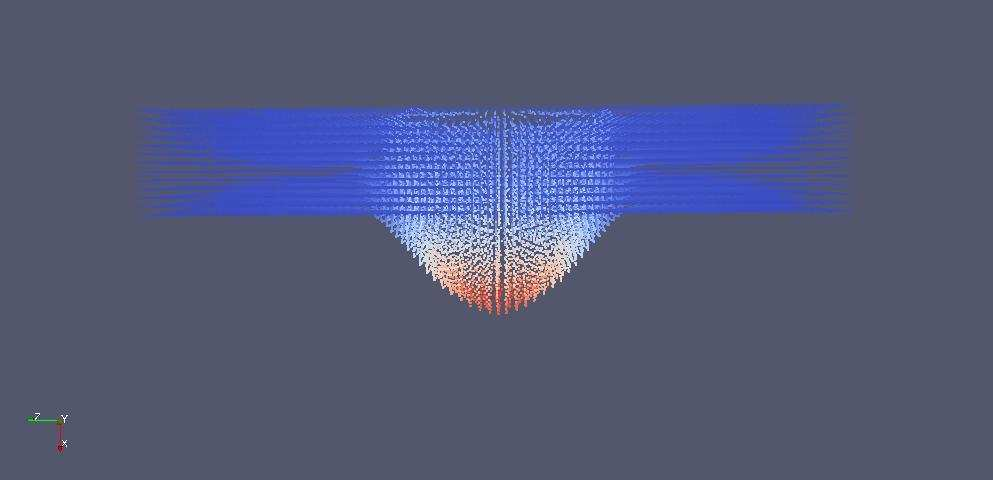
\includegraphics[width=0.8\textwidth]{img/sph_0.png}
    \caption{Общий вид. SPH. Удар под углом 0 градусов}

    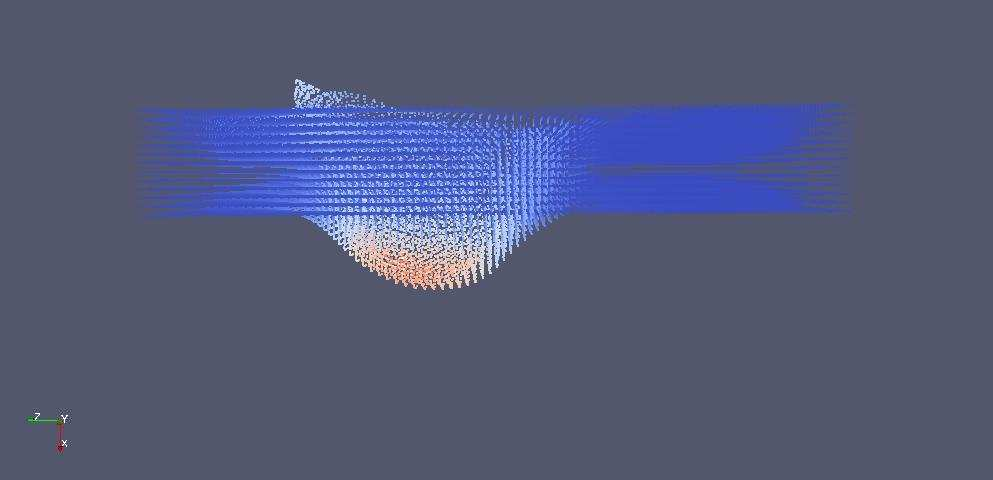
\includegraphics[width=0.8\textwidth]{img/sph_30.png}
    \caption{Общий вид. SPH. Удар под углом 30 градусов}

    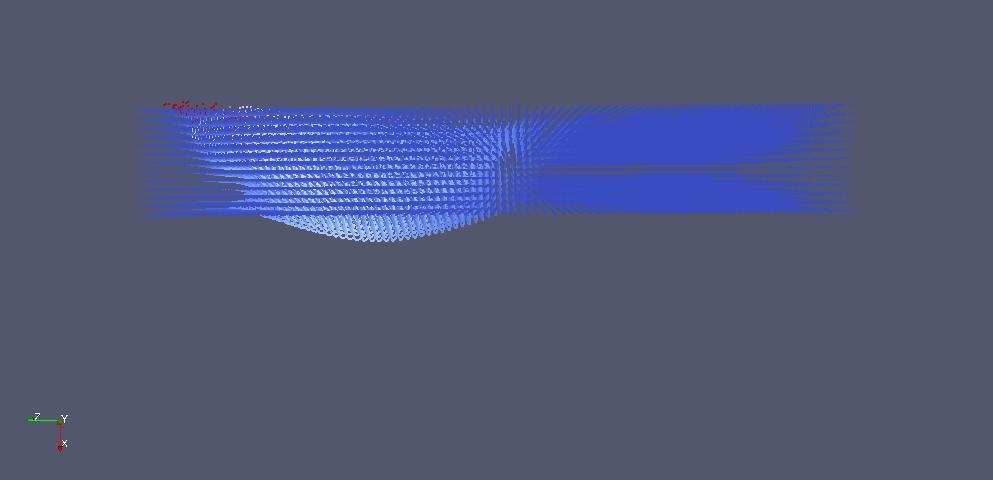
\includegraphics[width=0.8\textwidth]{img/sph_60.png}
    \caption{Общий вид. SPH. Удар под углом 60 градусов}
\end{figure}

Сразу следует отметить, что аналитическое решение и эксперименты по прострелу бронижилетов дают однозначный результат:
при косом ударе пробитие лучше.
В данном расчёте данный результат не воспроизводится.

\section{Моделирование мембраны}\label{sec:model-membrane}
Моделирование мембраны осуществлялось с помощью пакета Comsol Multiphysics.
В результате его работы были получены следующие решения: \picref{pic:comsol-example-1}.

\begin{figure}[H]
    \centering
    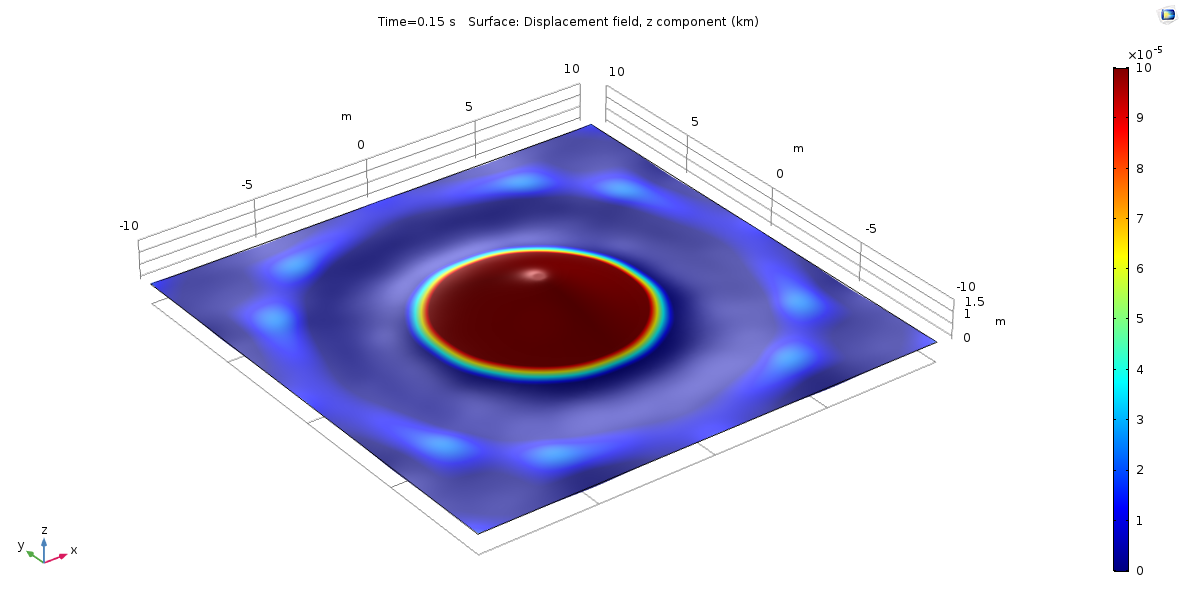
\includegraphics[width=0.8\textwidth]{img/comsol/example_1.png}
    \caption{}
    \label{pic:comsol-example-1}
\end{figure}

Данное решение хорошо описывает ожидаемое поведение тканного пакета, но, к сожалению, не даёт простого способа
получить интересующие нас данные по динамике, в частности скорости волнового фронта.

Это приводит нас к необходимости применить методы расчёта для отдельных нитей.

\section{Моделирование гибкой нити}\label{sec:model-fibers}
Для моделирования системы гибких нитей была написана программа~\ref{ch:program} реализующая метод
<<крест-колокол>>~\cite{rakhmatulin}.

Примеры результатов работы данной программы: \picref{pic:fiber-example-overview},
\picref{pic:fiber-example-top}, \picref{pic:fiber-example-bottom},
\picref{pic:fiber-example-side}, \picref{pic:fiber-example-slice}.

\begin{figure}[H]
    \centering
    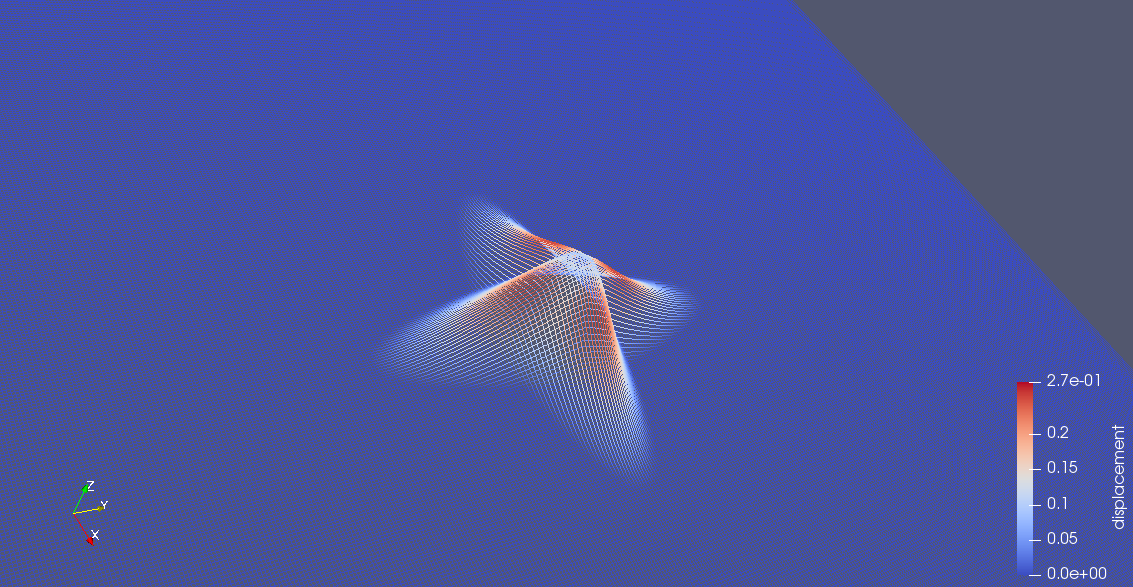
\includegraphics[width=0.8\textwidth]{img/fiber/example_overview.png}
    \caption{Общий вид}
    \label{pic:fiber-example-overview}
\end{figure}

\begin{figure}[H]
    \centering
    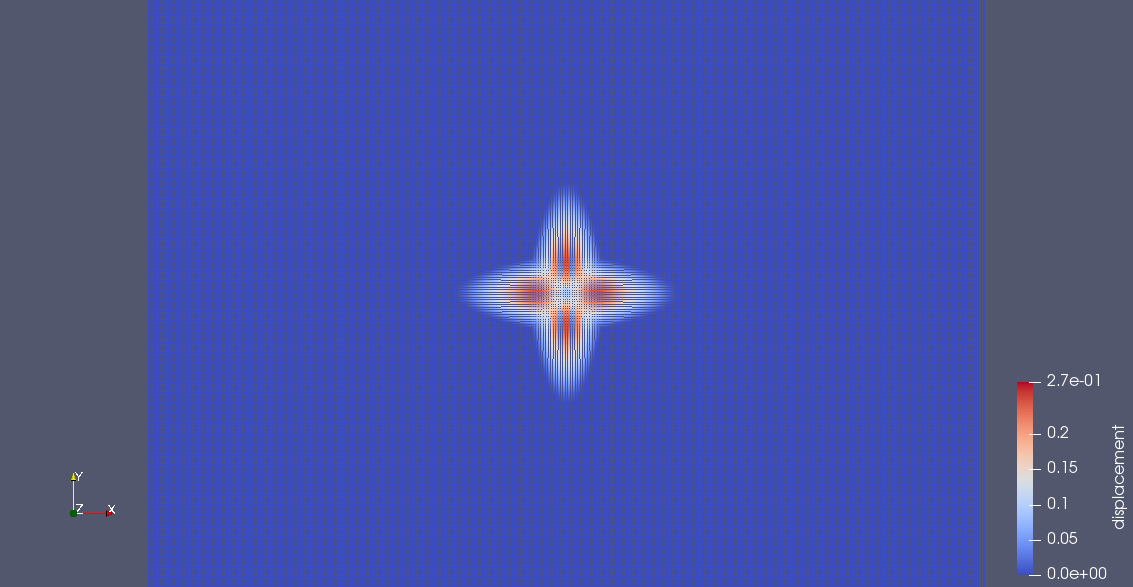
\includegraphics[width=0.8\textwidth]{img/fiber/example_top.png}
    \caption{Вид сверху}
    \label{pic:fiber-example-top}
\end{figure}

\begin{figure}[H]
    \centering
    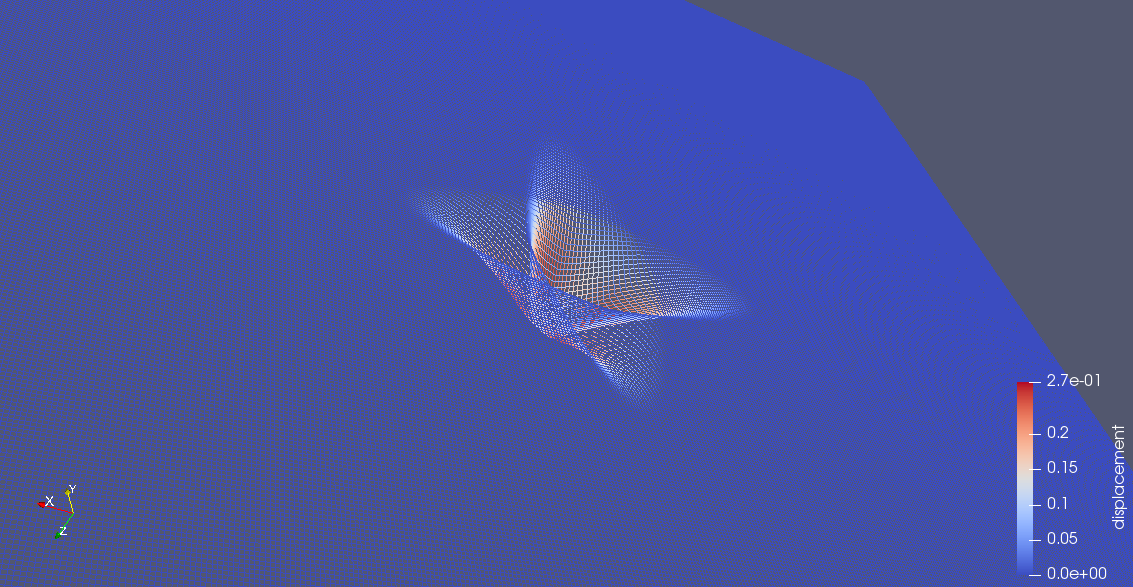
\includegraphics[width=0.8\textwidth]{img/fiber/example_bottom.png}
    \caption{Вид снизу. Виден прогиб ткани в центре.}
    \label{pic:fiber-example-bottom}
\end{figure}

\begin{figure}[H]
    \centering
    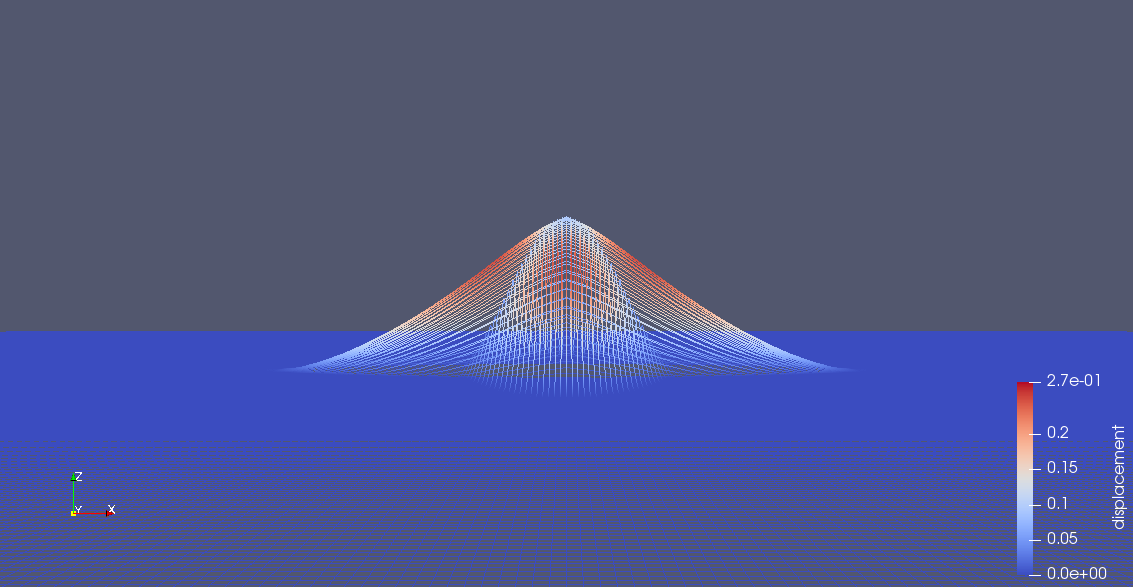
\includegraphics[width=0.8\textwidth]{img/fiber/example_side.png}
    \caption{Вид вдоль нитей}
    \label{pic:fiber-example-side}
\end{figure}

\begin{figure}[H]
    \centering
    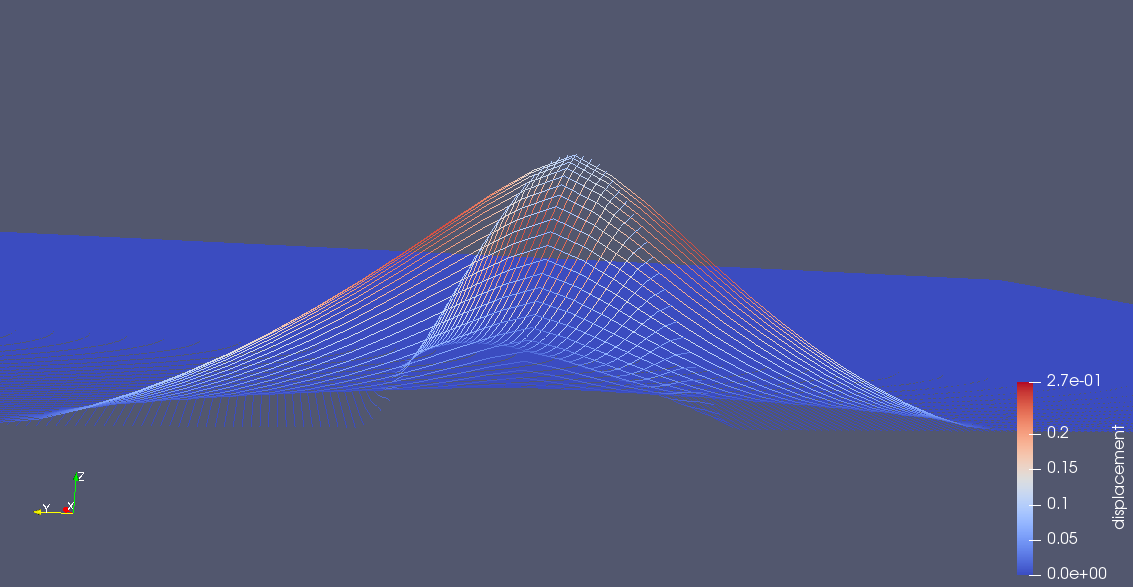
\includegraphics[width=0.8\textwidth]{img/fiber/example_slice.png}
    \caption{Срез вдоль нитей. Видно расслоение утка и основы.}
    \label{pic:fiber-example-slice}
\end{figure}


Большая часть расчётов при различных постановках приводится в~\ref{ch:results}.
